\newpage
\section{Cálculos sobre vehículos}
\label{anexo_calculos_sobre_vehiculos}

Este anexo contiene todos los cálculos necesarios para realizar el análisis completo de los distintos vehículos viables, para todos ellos se ha procedido al estudio de dos casos distintos.

El primero de ellos, hace referencia al supuesto en el que se realizan  pedidos de forma individualizada, con un trayecto medio de 5 \glssymbol{km} y un tiempo de reparto de 5 minutos. El segundo caso, alude al supuesto en el que se realicen dos pedidos por reparto, con un trayecto medio de 7,5 \glssymbol{km} y se empleen 10 minutos en el reparto. Esta información queda plasmada en la tabla \autoref{tabla:tabla_datos_comunes}, en la cual también se recogen otros datos pertinentes comunes a los diversos cálculos contenidos en el anexo.


\begin{table}[H]
\centering
\begin{tabular}{|l|c|}
\hline

%Impuestos en motocicletas
%Seguro en motocicletas
%Seguro en patinetes
%Mantenimiento motocicletas eléctricas
%Mantenimiento 
%Equipamiento para motocicletas
%Equipamiento para patinetes
Precio medio de la   luz (\glssymbol{euro}/\glssymbol{kilovatiohora}) & 0,11193 \\ \hline
Precio medio de la gasolina (\glssymbol{euro}/\glssymbol{litros}) & 1,38 \\ \hline
Distancia a recorrer por reparto (\glssymbol{km}) & 5 \\ \hline
Distancia a recorrer por reparto doble (\glssymbol{km}) & 7,5 \\ \hline
Tiempo por reparto (\glssymbol{minuto}) & 5 \\ \hline
Tiempo por reparto doble (\glssymbol{minuto}) & 10 \\ \hline
Precio equipamiento patinetes (\glssymbol{euro}) & 114,76 \\ \hline
Precio equipamiento motocicletas/ciclomotores (\glssymbol{euro}) & 190,58 \\ \hline
Seguro en patinetes (\glssymbol{euro}) & 35 \\ \hline
Seguro en motocicletas/ciclomotores (\glssymbol{euro}) & 265 \\ \hline
Impuesto circulación patinetes (\glssymbol{euro}) & 0 \\ \hline
Impuesto circulación motocicletas/ciclomotores (\glssymbol{euro}) & 8,55 \\ \hline
Impuesto matriculación patinetes (\glssymbol{euro}) & 0 \\ \hline
\end{tabular}
%Impuesto matriculación motocicletas/ciclomotores (\glssymbol{euro}) & 0 \\ \hline
% Impuesto circulación motocicletas de 125 \glssymbol{cc} (\glssymbol{euro}) & 99,77 \\ \hline
\caption{Datos comunes para los distintos vehículos viables.}
\label{tabla:tabla_datos_comunes}
\end{table}


Además de los dos escenarios distintos, se valorarán cuatro franjas horarias de reparto y los dos intervalos semanales que se plantean como datos de estudio. El primer escenario que se estudia abarca de lunes a jueves, con primer turno de trabajo de nueve de la mañana a ocho de la tarde, y segundo turno de 8 de la tarde a doce de la noche, recogidos en la \autoref{tab:distribucion de reparto}. La empresa demandante nos proporciona como información un reparto homogéneo en el tiempo y por cada intervalo correspondiente. Se observa que el volumen de repartos es mayor los fines de semana que en el resto, por lo que se espera obtener en los resultados una mayor cantidad de vehículos en esos tramos.

Otro limitante a tener en cuenta es la autonomía del vehículo, por lo que se calcula el tiempo que se encuentra circulando en carretera con ayuda de la velocidad estimada y la distancia de recorrido. Una vez obtenido el tiempo en carretera, se le incluyen el tiempo de reparto, donde el repartidor se desplaza de la calle a la vivienda, entrega el pedido, cobra el importe y regresa al vehículo.

Con el tiempo estimado por pedido y el tiempo total de la franja horaria se determina el número de pedidos que podría realizar una persona sin tener en cuenta las limitaciones de la autonomía. Según el valor que se obtenga, se compara con el número de pedidos que son necesario cumplir, y se añaden tantos vehículos como sean necesarios hasta igualar o superar la cifra de pedidos.

A partir de toda la información anterior, se puede calcular el tiempo que tardará el vehículo en necesitar una recarga de combustible o batería, permitiendo así obtener el número de vehículos extraordinarios en caso de estar trabajando con los modelos eléctricos.

Así pues, conociendo la cantidad de vehículos en total, se podrá estimar la cantidad de vehículos que debe adquirir la empresa para cumplir con la demanda de cada una de las franjas de este estudio.

Por otro lado, se debe tener en cuenta en los cálculos el tiempo de repostaje o recarga del vehículo. En el caso de vehículos a gasolina no tendrá un valor considerable, ya que el tiempo de llenado de depósito no supera los pocos minutos. Por el contrario, en los vehículos eléctricos, en el supuesto que la empresa opte por recargas de baterías del vehículo, se tendrá en consideración el tiempo donde no puede ser empleado para los repartos.

\subsection{Ciclomotor gasolina 50cc, KYMCO Agility Carry 50 E5}
\label{Ciclomotor gasolina 50cc, KYMCO Agility Carry 50}
%% kilómetro que recorre la moto
%% litros que puede llevar
%% precio de la moto
Entre los distintos ciclomotores del mercado, el modelo KYMCO Agility Carry 50 E5 resulta ser uno de los más ventajosos. A continuación, en la \autoref{tab:Datos ciclomotores de gasolina} se indican las características necesarias para realizar un análisis económico del vehículo.

\begin{table}[H]
\centering
\begin{tabular}{|l|c|}
\hline
Alcance máximo con   carga completa    & 350-300 \glssymbol{km} \\ \hline
Alcance estimado con carga completa    & 300 \glssymbol{km}    \\ \hline
Velocidad máxima alcanzable            & 60 \glssymbol{km}/\glssymbol{hora}  \\ \hline
Velocidad media estimada               & 40 \glssymbol{km}/\glssymbol{hora}  \\ \hline
\end{tabular}
\caption{Datos ciclomotores de gasolina.}
\label{tab:Datos ciclomotores de gasolina}
\end{table}

A efectos prácticos, la \autoref{tab:Análisis detallado motocicletas de gasolina, viajes de 5 km} coincide con la \autoref{tab:Análisis detallado ciclomotores de gasolina, viajes de 5 km} y la \autoref{tab:Análisis detallado motocicletas de gasolina, viajes de 7,5 km} es idéntica a la \autoref{tab:Análisis detallado ciclomotores de gasolina, viajes de 7,5 km}, debido a que con números relativamente pequeños, las características diferentes entre los modelos KYMCO Agility Carry 50 E5 y KYMCO Agility Carry 125 apenas interfieren en el estudio de la entrega de pedidos. 

\begin{table}[H]
\centering
\begin{tabular}{l|c|c|c|c|}
\cline{2-5}
 & \begin{tabular}[c]{@{}c@{}}TRAMO \\ HORARIO 1\end{tabular} & \begin{tabular}[c]{@{}c@{}}TRAMO \\ HORARIO 2\end{tabular} & \begin{tabular}[c]{@{}c@{}}TRAMO \\ HORARIO 3\end{tabular} & \begin{tabular}[c]{@{}c@{}}TRAMO \\ HORARIO 4\end{tabular} \\ \cline{2-5} 
 & \begin{tabular}[c]{@{}c@{}}Lunes-Jueves \\ (9:00-20:00)\end{tabular} & \begin{tabular}[c]{@{}c@{}}Lunes-Jueves \\ (20:00-0:00)\end{tabular} & \begin{tabular}[c]{@{}c@{}}Viernes-Domingo \\ 9:00-20:00)\end{tabular} & \begin{tabular}[c]{@{}c@{}}Viernes-Domingo \\ 20:00-1:00)\end{tabular} \\ \hline
\multicolumn{1}{|l|}{Nº pedidos} & 40 & 50 & 60 & 120 \\ \hline
\multicolumn{1}{|l|}{\begin{tabular}[c]{@{}l@{}}Distancia total \\ a recorrer (\glssymbol{km})\end{tabular}} & 200 & 250 & 300 & 600 \\ \hline
\multicolumn{1}{|l|}{\begin{tabular}[c]{@{}l@{}}Tiempo total de \\ reparto (\glssymbol{minuto})\end{tabular}} & 660 & 240 & 660 & 300 \\ \hline
\multicolumn{1}{|l|}{\begin{tabular}[c]{@{}l@{}}Tiempo estimado por \\ pedido (\glssymbol{minuto}/pedido)\end{tabular}} & 12,5 & 12,5 & 12,5 & 12,5 \\ \hline
\multicolumn{1}{|l|}{\begin{tabular}[c]{@{}l@{}}Nº pedidos realizables \\ por vehículo\end{tabular}} & 52,8 & 19,2 & 52,8 & 24 \\ \hline
\multicolumn{1}{|l|}{\begin{tabular}[c]{@{}l@{}}Nº vehículos \\ simultáneos necesarios\end{tabular}} & 1 & 3 & 2 & 5 \\ \hline
\multicolumn{1}{|l|}{\begin{tabular}[c]{@{}l@{}}Nº de turnos \\ de vehículos\end{tabular}} & 1 & 1 & 1 & 1 \\ \hline
\multicolumn{1}{|l|}{\begin{tabular}[c]{@{}l@{}}Nº vehículos \\ totales necesarios\end{tabular}} & 1 & 3 & 2 & 5 \\ \hline
\end{tabular}
\caption{Análisis detallado ciclomotores de gasolina, viajes de 5 km.}
\label{tab:Análisis detallado ciclomotores de gasolina, viajes de 5 km}
\end{table}



\begin{table}[H]
\centering
\begin{tabular}{l|c|c|c|c|}
\cline{2-5}
 & \begin{tabular}[c]{@{}c@{}}TRAMO \\ HORARIO 1\end{tabular} & \begin{tabular}[c]{@{}c@{}}TRAMO \\ HORARIO 2\end{tabular} & \begin{tabular}[c]{@{}c@{}}TRAMO \\ HORARIO 3\end{tabular} & \begin{tabular}[c]{@{}c@{}}TRAMO \\ HORARIO 4\end{tabular} \\ \cline{2-5} 
 & \begin{tabular}[c]{@{}c@{}}Lunes-Jueves \\ (9:00-20:00)\end{tabular} & \begin{tabular}[c]{@{}c@{}}Lunes-Jueves \\ (20:00-0:00)\end{tabular} & \begin{tabular}[c]{@{}c@{}}Viernes-Domingo \\ 9:00-20:00)\end{tabular} & \begin{tabular}[c]{@{}c@{}}Viernes-Domingo \\ 20:00-1:00)\end{tabular} \\ \hline
\multicolumn{1}{|l|}{Nº pedidos} & 20 & 25 & 30 & 60 \\ \hline
\multicolumn{1}{|l|}{\begin{tabular}[c]{@{}l@{}}Distancia total \\ a recorrer (\glssymbol{km})\end{tabular}} & 150 & 187,5 & 225 & 450 \\ \hline
\multicolumn{1}{|l|}{\begin{tabular}[c]{@{}l@{}}Tiempo total de \\ reparto (\glssymbol{minuto})\end{tabular}} & 660 & 240 & 660 & 300 \\ \hline
\multicolumn{1}{|l|}{\begin{tabular}[c]{@{}l@{}}Tiempo estimado por \\ pedido (\glssymbol{minuto}/pedido)\end{tabular}} & 21,25 & 21,25 & 21,25 & 21,25 \\ \hline
\multicolumn{1}{|l|}{\begin{tabular}[c]{@{}l@{}}Nº pedidos realizables \\ por vehículo\end{tabular}} & 31 & 11 & 31 & 14 \\ \hline
\multicolumn{1}{|l|}{\begin{tabular}[c]{@{}l@{}}Nº vehículos \\ simultáneos necesarios\end{tabular}} & 1 & 3 & 1 & 5 \\ \hline
\multicolumn{1}{|l|}{\begin{tabular}[c]{@{}l@{}}Nº de turnos \\ de vehículos\end{tabular}} & 1 & 1 & 1 & 1 \\ \hline
\multicolumn{1}{|l|}{\begin{tabular}[c]{@{}l@{}}Nº vehículos \\ totales necesarios\end{tabular}} & 1 & 3 & 1 & 5 \\ \hline
\end{tabular}
\caption{Análisis detallado ciclomotores de gasolina, viajes de 7,5 km.}
\label{tab:Análisis detallado ciclomotores de gasolina, viajes de 7,5 km}
\end{table}

Los vehículos de gasolina no deben ser sustituidos pues su repostaje apenas supone tiempo y no se ha considerado en este estudio. Según la  \autoref{tab:Análisis detallado motocicletas de gasolina, viajes de 5 km} y la \autoref{tab:Análisis detallado motocicletas de gasolina, viajes de 7,5 km}, se deduce que son necesarios 5 vehículos para el tramo horario más desfavorable (cuello de botella) para las dos opciones contempladas.


Por último, a partir del número de vehículos necesarios, los datos de la \autoref{tab:Datos ciclomotores de gasolina}, los de la \autoref{tabla:tabla_datos_comunes} y otros datos de cálculo incluidos en la misma \autoref{tab:Presupuesto motillo Peter}, se ha elaborado un presupuesto de este modelo, tanto en un primer año como un a lo largo de 10 años.

\begin{table}[H]
\centering
\begin{tabular}{|l|c|}
\hline
N.º repostajes semanales caso 1 & 6 \\ \hline
N.º repostajes semanales caso 2 & 5 \\ \hline
Capacidad depósito del vehículo (\glssymbol{litros}) & 6 \\ \hline
Coste recarga unitario (\glssymbol{euro}) & 8,28 \\ \hline
Gasto semanal en  repostajes caso 1 (\glssymbol{euro}) & 41,40 \\ \hline
Gasto semanal en  repostajes caso 2 (\glssymbol{euro}) & 33,12 \\ \hline
Presupuesto anual en repostajes caso 1 (\glssymbol{euro}) & 2.152,80 \\ \hline
Presupuesto anual en repostajes caso 2 (\glssymbol{euro}) & 1.722,24 \\ \hline
Precio unitario/vehículo (\glssymbol{euro}) & 1.999 \\ \hline
Precio unitario mantenimiento (\glssymbol{euro}) & 239 \\ \hline
Reserva de sustitución por vehículo (\glssymbol{euro}) & 50 \\ \hline
Presupuesto para   vehículos primer año caso 1 (\glssymbol{euro}) & 16.052,70 \\ \hline
Presupuesto para vehículos primer año   caso 2 (\glssymbol{euro}) & 15.622,14 \\ \hline
Presupuesto para vehículos anual  caso 1 (\glssymbol{euro}) & 4.965,55 \\ \hline
Presupuesto para vehículos anual caso 2 (\glssymbol{euro}) & 4.534,99 \\ \hline
Presupuesto en vehículos a 10 años, caso 1 (\glssymbol{euro}) & 60.742,65 \\ \hline
Presupuesto en vehículos a 10 años, caso 2 (\glssymbol{euro}) & 56.437,05 \\ \hline
\end{tabular}
\caption{Presupuesto ciclomotor KYMCO Agility Carry 50 E5.}
\label{tab:Presupuesto motillo Peter}
\end{table}

\subsection{Motocicleta gasolina 125cc, KYMCO Agility Carry 125}
\label{sub_anexo_calculos_motocicleta}
En esta sección del anexo, se recogen los datos numéricos relativos a la motocicleta de gasolina KYMCO Agility Carry 125. Tomando como referencia datos de la
\autoref{tabla:tabla_datos_comunes}, se añaden especificaciones concretas del modelo en la tabla \autoref{tab:Datos motocileta de gasolina}.


\begin{table}[H]
\centering
\begin{tabular}{|l|c|}
\hline
Alcance máximo con   carga completa    & 250-300 \glssymbol{km} \\ \hline
Alcance estimado con carga completa    & 250 \glssymbol{km}    \\ \hline
Velocidad máxima alcanzable            & 120 \glssymbol{km}/\glssymbol{hora}  \\ \hline
Velocidad media estimada               & 40 \glssymbol{km}/\glssymbol{hora}  \\ \hline
\end{tabular}
\caption{Datos motocicleta de gasolina.}
\label{tab:Datos motocileta de gasolina}
\end{table}


Los dos casos a analizar están reflejados en la \autoref{tab:Análisis detallado motocicletas de gasolina, viajes de 5 km} y la \autoref{tab:Análisis detallado motocicletas de gasolina, viajes de 7,5 km}. Para el estudio de este tipo de vehículo, no es necesario realizar ninguna gráfica adicional a las tablas obtenidas, pues al ser un vehículo de gasolina, repostar implica un par de minutos y no es necesario ningún cambio de vehículo.


\begin{table}[H]
\centering
\begin{tabular}{l|c|c|c|c|}
\cline{2-5}
 & \begin{tabular}[c]{@{}c@{}}TRAMO \\ HORARIO 1\end{tabular} & \begin{tabular}[c]{@{}c@{}}TRAMO \\ HORARIO 2\end{tabular} & \begin{tabular}[c]{@{}c@{}}TRAMO \\ HORARIO 3\end{tabular} & \begin{tabular}[c]{@{}c@{}}TRAMO \\ HORARIO 4\end{tabular} \\ \cline{2-5} 
 & \begin{tabular}[c]{@{}c@{}}Lunes-Jueves \\ (9:00-20:00)\end{tabular} & \begin{tabular}[c]{@{}c@{}}Lunes-Jueves \\ (20:00-0:00)\end{tabular} & \begin{tabular}[c]{@{}c@{}}Viernes-Domingo \\ 9:00-20:00)\end{tabular} & \begin{tabular}[c]{@{}c@{}}Viernes-Domingo \\ 20:00-1:00)\end{tabular} \\ \hline
\multicolumn{1}{|l|}{Nº pedidos} & 40 & 50 & 60 & 120 \\ \hline
\multicolumn{1}{|l|}{\begin{tabular}[c]{@{}l@{}}Distancia total \\ a recorrer (\glssymbol{km})\end{tabular}} & 200 & 250 & 300 & 600 \\ \hline
\multicolumn{1}{|l|}{\begin{tabular}[c]{@{}l@{}}Tiempo total de \\ reparto (\glssymbol{minuto})\end{tabular}} & 660 & 240 & 660 & 300 \\ \hline
\multicolumn{1}{|l|}{\begin{tabular}[c]{@{}l@{}}Tiempo estimado por \\ pedido (\glssymbol{minuto}/pedido)\end{tabular}} & 12,5 & 12,5 & 12,5 & 12,5 \\ \hline
\multicolumn{1}{|l|}{\begin{tabular}[c]{@{}l@{}}Nº pedidos realizables \\ por vehículo\end{tabular}} & 52,8 & 19,2 & 52,8 & 24 \\ \hline
\multicolumn{1}{|l|}{\begin{tabular}[c]{@{}l@{}}Nº vehículos \\ simultáneos necesarios\end{tabular}} & 1 & 3 & 2 & 5 \\ \hline
\multicolumn{1}{|l|}{\begin{tabular}[c]{@{}l@{}}Nº de turnos \\ de vehículos\end{tabular}} & 1 & 1 & 1 & 1 \\ \hline
\multicolumn{1}{|l|}{\begin{tabular}[c]{@{}l@{}}Nº vehículos \\ totales necesarios\end{tabular}} & 1 & 3 & 2 & 5 \\ \hline
\end{tabular}
\caption{Análisis detallado motocicletas de gasolina, viajes de 5 km.}
\label{tab:Análisis detallado motocicletas de gasolina, viajes de 5 km}
\end{table}



\begin{table}[H]
\centering
\begin{tabular}{l|c|c|c|c|}
\cline{2-5}
 & \begin{tabular}[c]{@{}c@{}}TRAMO \\ HORARIO 1\end{tabular} & \begin{tabular}[c]{@{}c@{}}TRAMO \\ HORARIO 2\end{tabular} & \begin{tabular}[c]{@{}c@{}}TRAMO \\ HORARIO 3\end{tabular} & \begin{tabular}[c]{@{}c@{}}TRAMO \\ HORARIO 4\end{tabular} \\ \cline{2-5} 
 & \begin{tabular}[c]{@{}c@{}}Lunes-Jueves \\ (9:00-20:00)\end{tabular} & \begin{tabular}[c]{@{}c@{}}Lunes-Jueves \\ (20:00-0:00)\end{tabular} & \begin{tabular}[c]{@{}c@{}}Viernes-Domingo \\ 9:00-20:00)\end{tabular} & \begin{tabular}[c]{@{}c@{}}Viernes-Domingo \\ 20:00-1:00)\end{tabular} \\ \hline
\multicolumn{1}{|l|}{Nº pedidos} & 20 & 25 & 30 & 60 \\ \hline
\multicolumn{1}{|l|}{\begin{tabular}[c]{@{}l@{}}Distancia total \\ a recorrer (\glssymbol{km})\end{tabular}} & 150 & 187,5 & 225 & 450 \\ \hline
\multicolumn{1}{|l|}{\begin{tabular}[c]{@{}l@{}}Tiempo total de \\ reparto (\glssymbol{minuto})\end{tabular}} & 660 & 240 & 660 & 300 \\ \hline
\multicolumn{1}{|l|}{\begin{tabular}[c]{@{}l@{}}Tiempo estimado por \\ pedido (\glssymbol{minuto}/pedido)\end{tabular}} & 21,25 & 21,25 & 21,25 & 21,25 \\ \hline
\multicolumn{1}{|l|}{\begin{tabular}[c]{@{}l@{}}Nº pedidos realizables \\ por vehículo\end{tabular}} & 31 & 11 & 31 & 14 \\ \hline
\multicolumn{1}{|l|}{\begin{tabular}[c]{@{}l@{}}Nº vehículos \\ simultáneos necesarios\end{tabular}} & 1 & 3 & 1 & 5 \\ \hline
\multicolumn{1}{|l|}{\begin{tabular}[c]{@{}l@{}}Nº de turnos \\ de vehículos\end{tabular}} & 1 & 1 & 1 & 1 \\ \hline
\multicolumn{1}{|l|}{\begin{tabular}[c]{@{}l@{}}Nº vehículos \\ totales necesarios\end{tabular}} & 1 & 3 & 1 & 5 \\ \hline
\end{tabular}
\caption{Análisis detallado motocicletas de gasolina, viajes de 7,5 km.}
\label{tab:Análisis detallado motocicletas de gasolina, viajes de 7,5 km}
\end{table}

En resumen, de este modelo serían necesarios cinco vehículos para realizar satisfactoriamente todos los pedidos deseados en ambos casos estudiados.
En cuanto al presupuesto, queda recogido en la \autoref{tab:Presupuesto motocicletas de gasolina}.

\begin{table}[H]
\centering
\begin{tabular}{|l|c|}
\hline
N.º repostajes semanales caso 1 & 6 \\ \hline
N.º repostajes semanales caso 2 & 5 \\ \hline
Capacidad depósito del vehículo (\glssymbol{litros}) & 6,5 \\ \hline
Coste recarga unitario (\glssymbol{euro}) & 8,28 \\ \hline
Gasto semanal en  repostajes caso 1 (\glssymbol{euro}) & 53,82 \\ \hline
Gasto semanal en  repostajes caso 2 (\glssymbol{euro}) & 44,85 \\ \hline
Presupuesto anual en repostajes caso 1 (\glssymbol{euro}) & 2.798,64 \\ \hline
Presupuesto anual en repostajes caso 2 (\glssymbol{euro}) & 2.332,20 \\ \hline
Precio unitario/vehículo (\glssymbol{euro}) & 2.149 \\ \hline
Precio unitario mantenimiento (\glssymbol{euro}) & 239 \\ \hline
Reserva de sustitución por vehículo (\glssymbol{euro}) & 100 \\ \hline
Presupuesto para   vehículos primer año caso 1 (\glssymbol{euro}) & 18.058,14 \\ \hline
Presupuesto para vehículos primer año   caso 2 (\glssymbol{euro}) & 17.591,70 \\ \hline
Presupuesto para vehículos anual  caso 1 (\glssymbol{euro}) & 5.861,39 \\ \hline
Presupuesto para vehículos anual caso 2 (\glssymbol{euro}) & 5.394,95 \\ \hline
Presupuesto en vehículos a 10 años, caso 1 (\glssymbol{euro}) & 70.810,65 \\ \hline
Presupuesto en vehículos a 10 años, caso 2 (\glssymbol{euro}) & 66.146,25 \\ \hline
\end{tabular}
\caption{Presupuesto motocicletas de gasolina.}
\label{tab:Presupuesto motocicletas de gasolina}
\end{table}

%x9" y las expresiones "z3" y "z4", se ha calculado que a lo largo de 10 años sería necesario invertir un total de 60.000 \glssymbol{euro}, unos 6.000 \glssymbol{euro} anuales aproximadamente. 

% Tabla x9

%\begin{equation}
%  16489,81+5234,81*9=63.603,1 \text{ \glssymbol{euro}} 
%\end{equation}

%\begin{equation}
%  16.043,65+4.788,65*9=59.141,5 \text{ \glssymbol{euro}}
%\end{equation}


\subsection{Motocicleta eléctrica, Askoll eS1}
\label{sub_anexo_calculos_motocicleta_eléctrica}
A continuación, se han recopilado los datos numéricos referentes a la motocicleta eléctrica Askoll eS1. Usando la de la tabla \autoref{tabla:tabla_datos_comunes} y los datos específicos del modelo de la \autoref{tabla: Datos_concretos_moto_electrica}, se han determinado el mínimo número de vehículos de este modelo necesarios para las dos hipótesis propuestas y los cuatro tramos horarios asignados.
%\textwidth
\begin{table}[H]
\centering
%\resizebox{}{!}{
\begin{tabular}{|l|c|}
\hline
Alcance máximo con   carga completa    & 100-120 \glssymbol{km} \\ \hline
Alcance estimado con carga completa    & 100 \glssymbol{km}    \\ \hline
Velocidad máxima alcanzable            & 45 \glssymbol{velocidad}  \\ \hline
Velocidad media estimada               & 40 \glssymbol{velocidad}  \\ \hline
Duración recarga            & 6 \glssymbol{hora} \\ \hline
\end{tabular}
\caption{Datos motocicleta eléctrica.}
\label{tabla: Datos_concretos_moto_electrica}
\end{table}


% Tabla x11
\begin{table}[H]
\centering
\resizebox{\textwidth}{!}{
\begin{tabular}{l|c|c|c|c|}
\cline{2-5}
 & \begin{tabular}[c]{@{}c@{}}TRAMO \\ HORARIO 1\end{tabular} & \begin{tabular}[c]{@{}c@{}}TRAMO \\ HORARIO 2\end{tabular} & \begin{tabular}[c]{@{}c@{}}TRAMO \\ HORARIO 3\end{tabular} & \begin{tabular}[c]{@{}c@{}}TRAMO \\ HORARIO 4\end{tabular} \\ \cline{2-5} 
 & \begin{tabular}[c]{@{}c@{}}Lunes-Jueves \\ (9:00-20:00)\end{tabular} & \begin{tabular}[c]{@{}c@{}}Lunes-Jueves \\ (20:00-0:00)\end{tabular} & \begin{tabular}[c]{@{}c@{}}Lunes-Jueves \\ 9:00-20:00)\end{tabular} & \begin{tabular}[c]{@{}c@{}}Viernes-Domingo \\ 20:00-1:00)\end{tabular} \\ \hline
\multicolumn{1}{|l|}{N.º pedidos} & 40 & 50 & 60 & 120 \\ \hline
\multicolumn{1}{|l|}{\begin{tabular}[c]{@{}l@{}}Distancia total \\ a recorrer (\glssymbol{km})\end{tabular}} & 200 & 250 & 300 & 600 \\ \hline
\multicolumn{1}{|l|}{\begin{tabular}[c]{@{}l@{}}Tiempo total de \\ reparto (\glssymbol{minuto})\end{tabular}} & 660 & 240 & 660 & 300 \\ \hline
\multicolumn{1}{|l|}{\begin{tabular}[c]{@{}l@{}}Tiempo estimado por \\ pedido (\glssymbol{minuto}/pedido)\end{tabular}} & 12,5 & 12,5 & 12,5 & 12,5 \\ \hline
\multicolumn{1}{|l|}{\begin{tabular}[c]{@{}l@{}}Nº pedidos realizables \\ por vehículo\end{tabular}} & 52,8 & 19,2 & 52,8 & 24,0 \\ \hline
\multicolumn{1}{|l|}{\begin{tabular}[c]{@{}l@{}}Nº vehículos \\ simultáneos necesarios\end{tabular}} & 1 & 3 & 2 & 5 \\ \hline
\multicolumn{1}{|l|}{\begin{tabular}[c]{@{}l@{}}Nº de turnos \\ de vehículos\end{tabular}} & 2 & 1 & 2 & 2 \\ \hline
\multicolumn{1}{|l|}{\begin{tabular}[c]{@{}l@{}}Nº vehículos \\ totales necesarios\end{tabular}} & 2 & 3 & 4 & 6 \\ \hline
\end{tabular}}
\caption{Estudio de pedidos para motocicletas eléctricas en viajes de 5 km.}
\label{tab:Estudio de pedidos para motocicletas eléctricas en viajes de 5 km}
\end{table}


\begin{table}[H]
\centering
\resizebox{\textwidth}{!}{
\begin{tabular}{l|c|c|c|c|}
\cline{2-5}
 & \begin{tabular}[c]{@{}c@{}}TRAMO \\ HORARIO 1\end{tabular} & \begin{tabular}[c]{@{}c@{}}TRAMO \\ HORARIO 2\end{tabular} & \begin{tabular}[c]{@{}c@{}}TRAMO \\ HORARIO 3\end{tabular} & \begin{tabular}[c]{@{}c@{}}TRAMO \\ HORARIO 4\end{tabular} \\ \cline{2-5} 
 & \begin{tabular}[c]{@{}c@{}}Lunes-Jueves \\ (9:00-20:00)\end{tabular} & \begin{tabular}[c]{@{}c@{}}Lunes-Jueves \\ (20:00-0:00)\end{tabular} & \begin{tabular}[c]{@{}c@{}}Viernes-Domingo \\ 9:00-20:00)\end{tabular} & \begin{tabular}[c]{@{}c@{}}Viernes-Domingo \\ 20:00-1:00)\end{tabular} \\ \hline
\multicolumn{1}{|l|}{Nº pedidos} & 20 & 25 & 30 & 60 \\ \hline
\multicolumn{1}{|l|}{\begin{tabular}[c]{@{}l@{}}Distancia total \\ a recorrer (\glssymbol{km})\end{tabular}} & 150 & 187,5 & 225 & 450 \\ \hline
\multicolumn{1}{|l|}{\begin{tabular}[c]{@{}l@{}}Tiempo total de \\ reparto (\glssymbol{minuto})\end{tabular}} & 660 & 240 & 660 & 300 \\ \hline
\multicolumn{1}{|l|}{\begin{tabular}[c]{@{}l@{}}Tiempo estimado por \\ pedido (\glssymbol{minuto}/pedido)\end{tabular}} & 21,3 & 21,3 & 21,3 & 21,3 \\ \hline
\multicolumn{1}{|l|}{\begin{tabular}[c]{@{}l@{}}Nº pedidos realizables \\ por vehículo\end{tabular}} & 31 & 11 & 31 & 14 \\ \hline
\multicolumn{1}{|l|}{\begin{tabular}[c]{@{}l@{}}Nº vehículos \\ simultáneos necesarios\end{tabular}} & 1 & 3 & 1 & 5 \\ \hline
\multicolumn{1}{|l|}{\begin{tabular}[c]{@{}l@{}}Nº de turnos \\ de vehículos\end{tabular}} & 2 & 1 & 3 & 1 \\ \hline
\multicolumn{1}{|l|}{\begin{tabular}[c]{@{}l@{}}Nº vehículos \\ totales necesarios\end{tabular}} & 2 & 3 & 3 & 5 \\ \hline
\end{tabular}}
\caption{Estudio de pedidos para motocicletas eléctricas en viajes de 7,5 km.}
\label{tab:Estudio de pedidos para motocicletas eléctricas en viajes de 7,5 km}
\end{table}


En función de los resultados recopilados en la \autoref{tab:Estudio de pedidos para motocicletas eléctricas en viajes de 5 km} y en la \autoref{tab:Estudio de pedidos para motocicletas eléctricas en viajes de 7,5 km}, son necesarias 10 motocicletas eléctricas para realizar el reparto de forma correcta en una de las hipótesis supuestas,8 para la segunda. Sin embargo, al tener en cuenta el tiempo que tarda este el modelo Askoll eS1 en cargarse completamente, el número de vehículos se puede reducir en ambas opciones, tal como se refleja en la \autoref{fig:motos_electricas_caso1} y en la \autoref{fig:motos_electricas_caso22}.

\begin{figure}[ht]
    \centering
    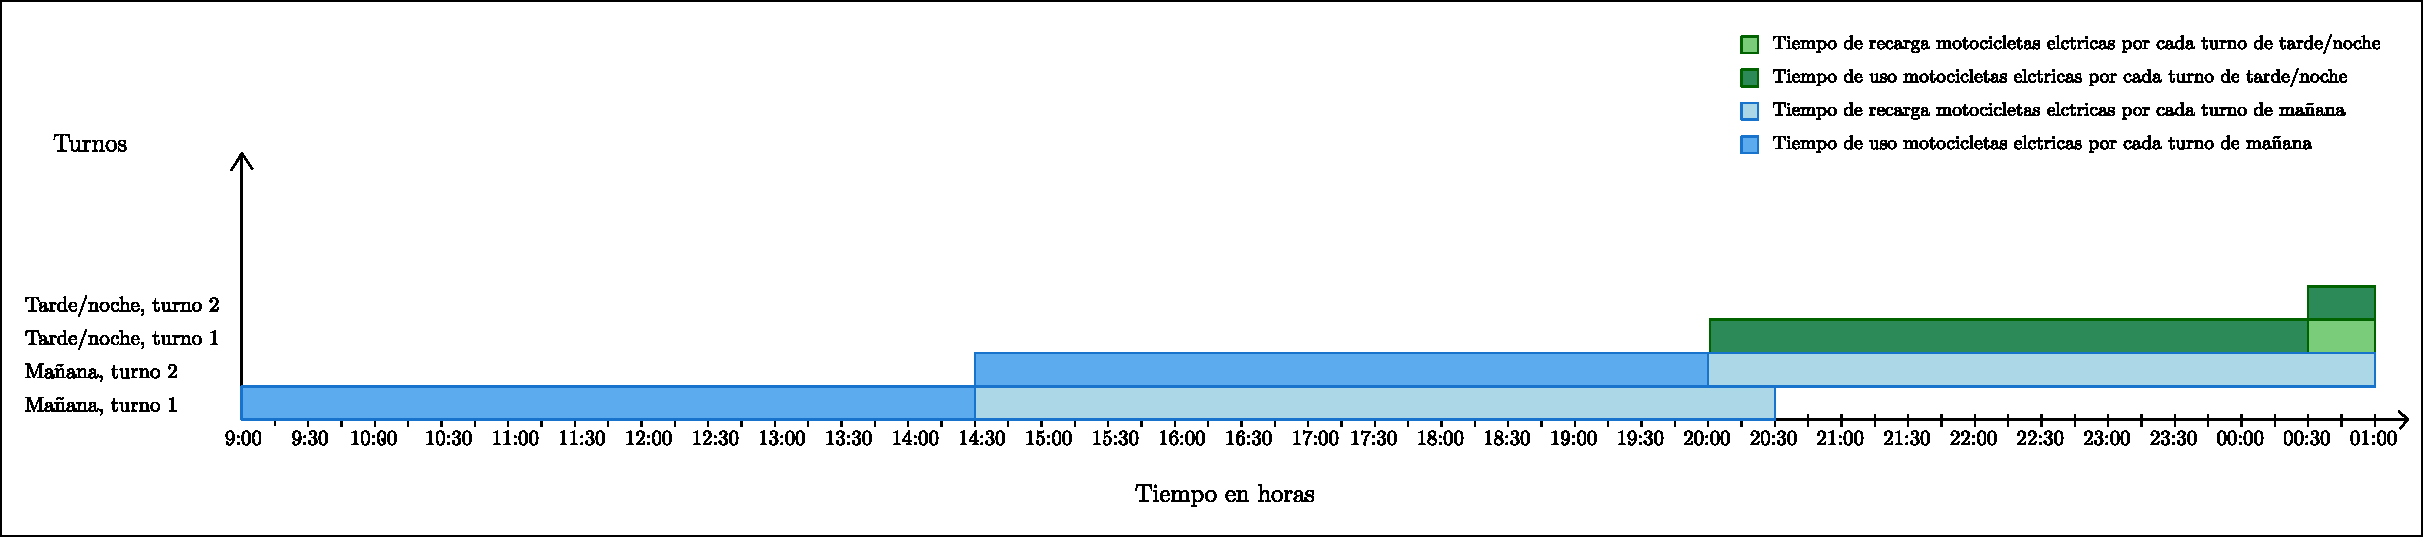
\includegraphics[width= \textwidth, height=12em]{archivos/caso1_motos_electricas.pdf}
    \caption{Representación turnos de motocicletas eléctricas en viajes de 5 \glssymbol{km}.}
    \label{fig:motos_electricas_caso1}
\end{figure}

La \autoref{fig:motos_electricas_caso1} muestra que durante el horario de mañana en el caso 1, tienen lugar 2 turnos de 2 vehículos cada uno (zona azul del gráfico). El color verde resalta el inicio del horario de tarde; en el primer turno se han de emplear 5 vehículos, mientras que en el segundo turno solo se emplea una motocicleta, la cual proviene del primer turno de la mañana.

\begin{figure}[ht]
    \centering
    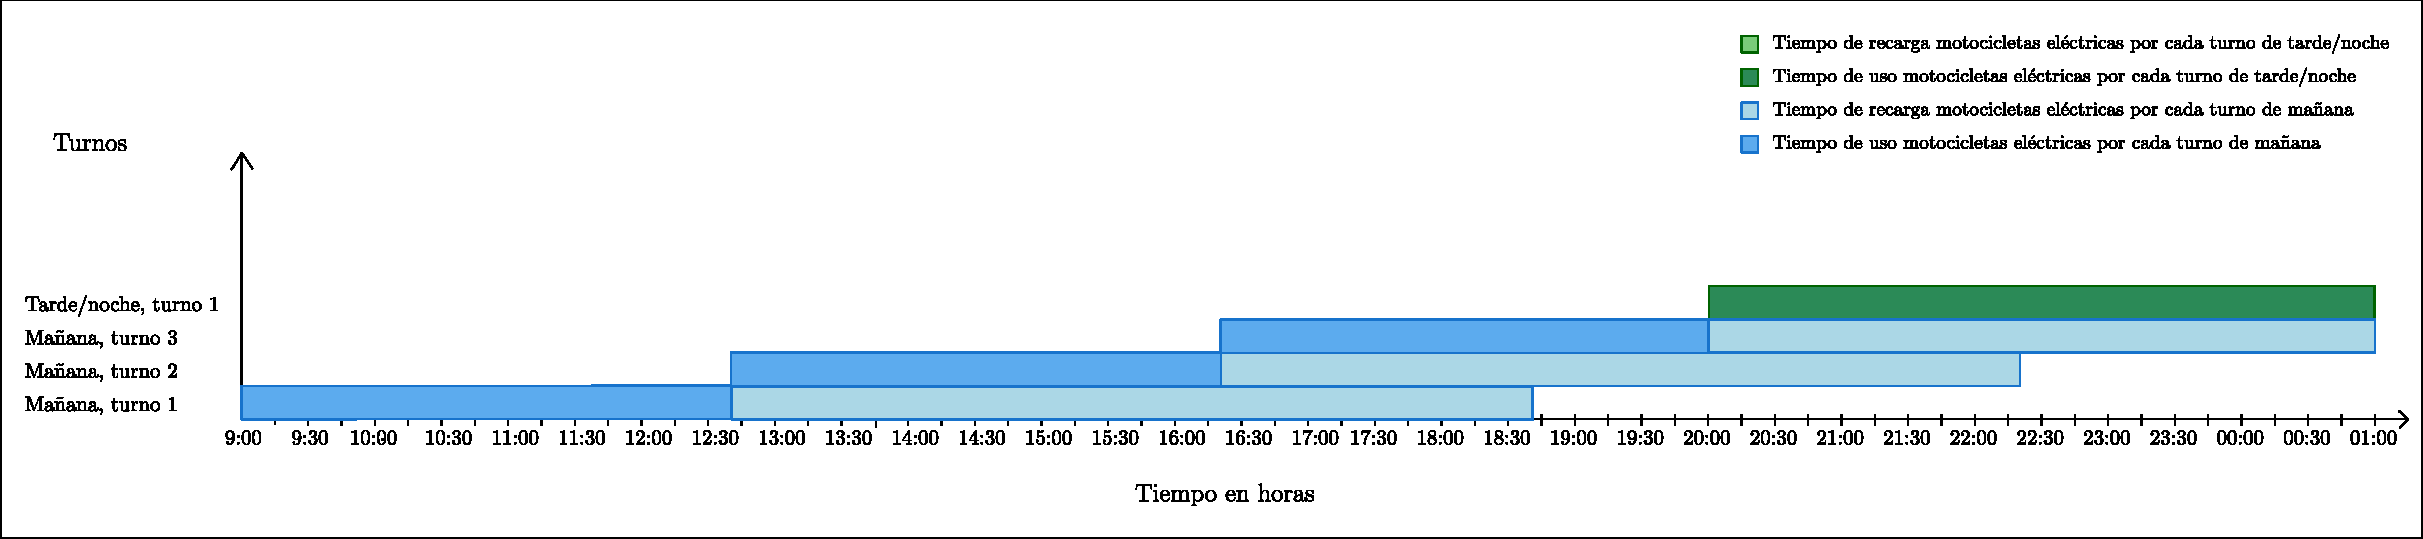
\includegraphics[width= \textwidth, height=12em]{archivos/caso2_motos_electricas.pdf}
    \caption{Representación turnos de motocicletas eléctricas en viajes de 7,5 \glssymbol{km}.}
    \label{fig:motos_electricas_caso22}
\end{figure}

Respecto a la \label{fig:motos_electricas_caso2}, que recoge la segunda hipótesis de repartos, se observan 4 turnos en total, 3 de mañana de 1 vehículo cada uno y 1 turno por la tarde de 5 vehículos simultáneos. En el turno de la tarde, como se debe reutilizar uno de los vehículos de la mañana solo son necesarios 7 vehículos en total. Es decir, se necesitan 9 motocicletas para el primer caso y 7 para el segundo caso de repartos.

Seguidamente, se agrupan los distintos gastos en la \autoref{tab:Estudio presupuestos modelo Askoll eS1}.

\begin{table}[H]
\centering
\begin{tabular}{|l|c|}
\hline
N.º recargas semanales caso 1 & 50 \\ \hline
N.º recargas semanales caso 2 & 44 \\ \hline
Capacidad batería vehículo (\glssymbol{kilovatiohora}) & 2,1 \\ \hline
Coste recarga unitario (\glssymbol{euro}) & 0,24 \\ \hline
Gasto semanal en  recargas caso 1 (\glssymbol{euro}) & 11,75 \\ \hline
Gasto semanal en  recargas caso 2 (\glssymbol{euro}) & 10,34 \\ \hline
Presupuesto anual en recargas caso 1 (\glssymbol{euro}) & 611,14 \\ \hline
Presupuesto anual en recargas caso 2 (\glssymbol{euro}) & 537,80 \\ \hline
Precio unitario/vehículo (\glssymbol{euro}) & 2.685 \\ \hline
Precio unitario mantenimiento (\glssymbol{euro}) & 126 \\ \hline
Reserva de sustitución por vehículo (\glssymbol{euro}) & 100 \\ \hline
Presupuesto para   vehículos primer año caso 1 (\glssymbol{euro}) & 30.475,64 \\ \hline
Presupuesto para vehículos primer año   caso 2 (\glssymbol{euro}) & 23.977,50 \\ \hline
Presupuesto para vehículos anual  caso 1 (\glssymbol{euro}) & 5.107,09 \\ \hline
Presupuesto para vehículos anual caso 2 (\glssymbol{euro}) & 4.034,65 \\ \hline
Presupuesto en vehículos a 10 años, caso 1 (\glssymbol{euro}) & 76.439,43 \\ \hline
Presupuesto en vehículos a 10 años, caso 2 (\glssymbol{euro}) & 60.289,36 \\ \hline
\end{tabular}
\caption{Estudio presupuestos modelo Askoll eS1.}
\label{tab:Estudio presupuestos modelo Askoll eS1}
\end {table}

%Empleando la tabla "x13" y las expresiones "z5" y "z6", se ha valorado que a lo largo de 10 años es necesario invertir un total de 40.000 \glssymbol{euro}, unos 4.000 \glssymbol{euro} anuales aproximadamente. 


%Análisis presupuestos modelo eSkoll

%\begin{equation}
%  15486,42+2898,52*9=41.573,1 \text{ \glssymbol{euro}}   
%\end{equation}
%\begin{equation}
%  15245,85+2657,95*9=39.167,4 \text{ \glssymbol{euro}}
%\end{equation}


\subsection{Infiniton CITYJam Pro}
\label{sub_anexo_calculos_patinete}

En la tabla \autoref{tabla: Datos_concretos_patinete} se han recogido las características específicas del modelo Infiniton CITYJam Pro con las que se van a trabajar para los cálculos correspondientes.


\begin{table}[H]
\centering
\begin{tabular}{|l|c|}
\hline
Alcance máximo con   carga completa    & 40-45 \glssymbol{km} \\ \hline
Alcance estimado con carga completa    & 40 \glssymbol{km}    \\ \hline
Velocidad máxima alcanzable            & 25 \glssymbol{velocidad}  \\ \hline
Velocidad media estimada               & 20 \glssymbol{velocidad}  \\ \hline
Duración recarga            & 6 \glssymbol{hora} 30 \glssymbol{minuto}  \\ \hline
\end{tabular}
\caption{Datos patinete eléctrico.}
\label{tabla: Datos_concretos_patinete}
\end{table}

Tal como se precisó anteriormente, se han supuesto dos hipótesis distintas a la hora de estudiar la distribución de los pedidos, lo que corresponde con la \autoref{tabla: analisis_detallado_patinete_5km} y la \autoref{tabla: analisis_detallado_patinete_7.5km}, respectivamente. En ellas, conocida la distancia total a recorrer por los vehículos, la duración de cada tramo horario considerado y los datos de la \autoref{tabla: Datos_concretos_patinete}, se ha obtenido el número de vehículos necesarios por cada uno de esos tramos.

% Tabla x3
\begin{table}[H]
\centering
\resizebox{\textwidth}{!}{
\begin{tabular}{l|c|c|c|c|}
\cline{2-5}
 & \begin{tabular}[c]{@{}c@{}}TRAMO \\ HORARIO 1\end{tabular} & \begin{tabular}[c]{@{}c@{}}TRAMO \\ HORARIO 2\end{tabular} & \begin{tabular}[c]{@{}c@{}}TRAMO \\ HORARIO 3\end{tabular} & \begin{tabular}[c]{@{}c@{}}TRAMO \\ HORARIO 4\end{tabular} \\ \cline{2-5} 
 & \begin{tabular}[c]{@{}c@{}}Lunes-Jueves \\ (9:00-20:00)\end{tabular} & \begin{tabular}[c]{@{}c@{}}Lunes-Jueves \\ (20:00-0:00)\end{tabular} & \begin{tabular}[c]{@{}c@{}}Viernes-Domingo \\ (9:00-20:00)\end{tabular} & \begin{tabular}[c]{@{}c@{}}Viernes-Domingo \\ (20:00-1:00)\end{tabular} \\ \hline
\multicolumn{1}{|l|}{Nº pedidos} & 40 & 50 & 60 & 120 \\ \hline
\multicolumn{1}{|l|}{\begin{tabular}[c]{@{}l@{}}Distancia total a \\ recorrer \glssymbol{km}\end{tabular}} & 200 & 250 & 300 & 600 \\ \hline
\multicolumn{1}{|l|}{\begin{tabular}[c]{@{}l@{}}Tiempo total de \\ reparto \glssymbol{minuto} \end{tabular}} & 660 & 240 & 660 & 300 \\ \hline
\multicolumn{1}{|l|}{\begin{tabular}[c]{@{}l@{}}Tiempo estimado \\ por pedido (\glssymbol{minuto}/pedido)\end{tabular}} & 20 & 20 & 20 & 20 \\ \hline
\multicolumn{1}{|l|}{\begin{tabular}[c]{@{}l@{}}Nº pedidos realizables \\ por vehículo\end{tabular}} & 33 & 12 & 33 & 15 \\ \hline
\multicolumn{1}{|l|}{\begin{tabular}[c]{@{}l@{}}Nº vehículos simultáneos \\ necesarios\end{tabular}} & 2 & 5 & 2 & 8 \\ \hline
\multicolumn{1}{|l|}{Nº de turnos de vehículos} & 3 & 2 & 4 & 2 \\ \hline
\multicolumn{1}{|l|}{\begin{tabular}[c]{@{}l@{}}Nº vehículos totales \\ necesarios\end{tabular}} & 6 & 10 & 8 & 16 \\ \hline
\end{tabular}}
\caption{Análisis detallado del reparto en patinete con viajes de 5 \glssymbol{km}.}
\label{tabla: analisis_detallado_patinete_5km}
\end{table}



\begin{table}[H]
\centering
\resizebox{\textwidth}{!}{
\begin{tabular}{l|c|c|c|c|}
\cline{2-5}
 & \begin{tabular}[c]{@{}c@{}}TRAMO \\ HORARIO 1\end{tabular} & \begin{tabular}[c]{@{}c@{}}TRAMO \\ HORARIO 2\end{tabular} & \begin{tabular}[c]{@{}c@{}}TRAMO \\ HORARIO 3\end{tabular} & \begin{tabular}[c]{@{}c@{}}TRAMO \\ HORARIO 4\end{tabular} \\ \cline{2-5} 
 & \begin{tabular}[c]{@{}c@{}}Lunes-Jueves \\ (9:00-20:00)\end{tabular} & \begin{tabular}[c]{@{}c@{}}Lunes-Jueves \\ (20:00-0:00)\end{tabular} & \begin{tabular}[c]{@{}c@{}}Viernes-Domingo \\ (9:00-20:00)\end{tabular} & \begin{tabular}[c]{@{}c@{}}Viernes-Domingo \\ (20:00-1:00)\end{tabular} \\ \hline
\multicolumn{1}{|l|}{Nº pedidos dobles} & 20 & 25 & 30 & 60 \\ \hline
\multicolumn{1}{|l|}{\begin{tabular}[c]{@{}l@{}}Distancia total a \\ recorrer (\glssymbol{km})\end{tabular}} & 150 & 187,5 & 225 & 450 \\ \hline
\multicolumn{1}{|l|}{\begin{tabular}[c]{@{}l@{}}Tiempo total de \\ reparto doble (\glssymbol{minuto})\end{tabular}} & 660 & 240 & 660 & 300 \\ \hline
\multicolumn{1}{|l|}{\begin{tabular}[c]{@{}l@{}}Tiempo estimado por \\ pedido doble (\glssymbol{minuto}/pedido)\end{tabular}} & 32,5 & 32,5 & 32,5 & 32,5 \\ \hline
\multicolumn{1}{|l|}{\begin{tabular}[c]{@{}l@{}}Nº pedidos dobles \\ realizables por vehículo\end{tabular}} & 20 & 7 & 20 & 9 \\ \hline
\multicolumn{1}{|l|}{\begin{tabular}[c]{@{}l@{}}Nº vehículos simultáneos \\ necesarios\end{tabular}} & 1 & 4 & 2 & 7 \\ \hline
\multicolumn{1}{|l|}{Nº de turnos de vehículos} & 4 & 2 & 3 & 2 \\ \hline
\multicolumn{1}{|l|}{\begin{tabular}[c]{@{}l@{}}Nº vehículos totales \\ necesarios\end{tabular}} & 4 & 8 & 6 & 14 \\ \hline
\end{tabular}}
\caption{Análisis detallado del reparto en patinete con viajes de 7,5 \glssymbol{km}.}
\label{tabla: analisis_detallado_patinete_7.5km}
\end{table}

En los cálculos realizados se ha tenido en cuenta también el tiempo de recarga del patinete, de un total de seis horas y treinta minutos, al igual que el tiempo de descarga, con su autonomía y velocidad.

Con base en los resultados numéricos obtenidos en la \autoref{tabla: analisis_detallado_patinete_5km}, sería necesaria una flota de 24 patinetes bajo la primera hipótesis y 20, para la segunda. No obstante, teniendo en cuenta las horas de uso de cada patinete y el tiempo de recarga de cada uno, se demuestra que solo son necesarios 20 patinetes para el primer caso estudiado, pues cuatro de los patines que se emplean durante el turno de día, pueden ser recargados y estar disponibles para su uso en el horario de tarde, como se observa en la \autoref{fig:patinetes_caso1}.

\begin{figure}[ht]
    \centering
    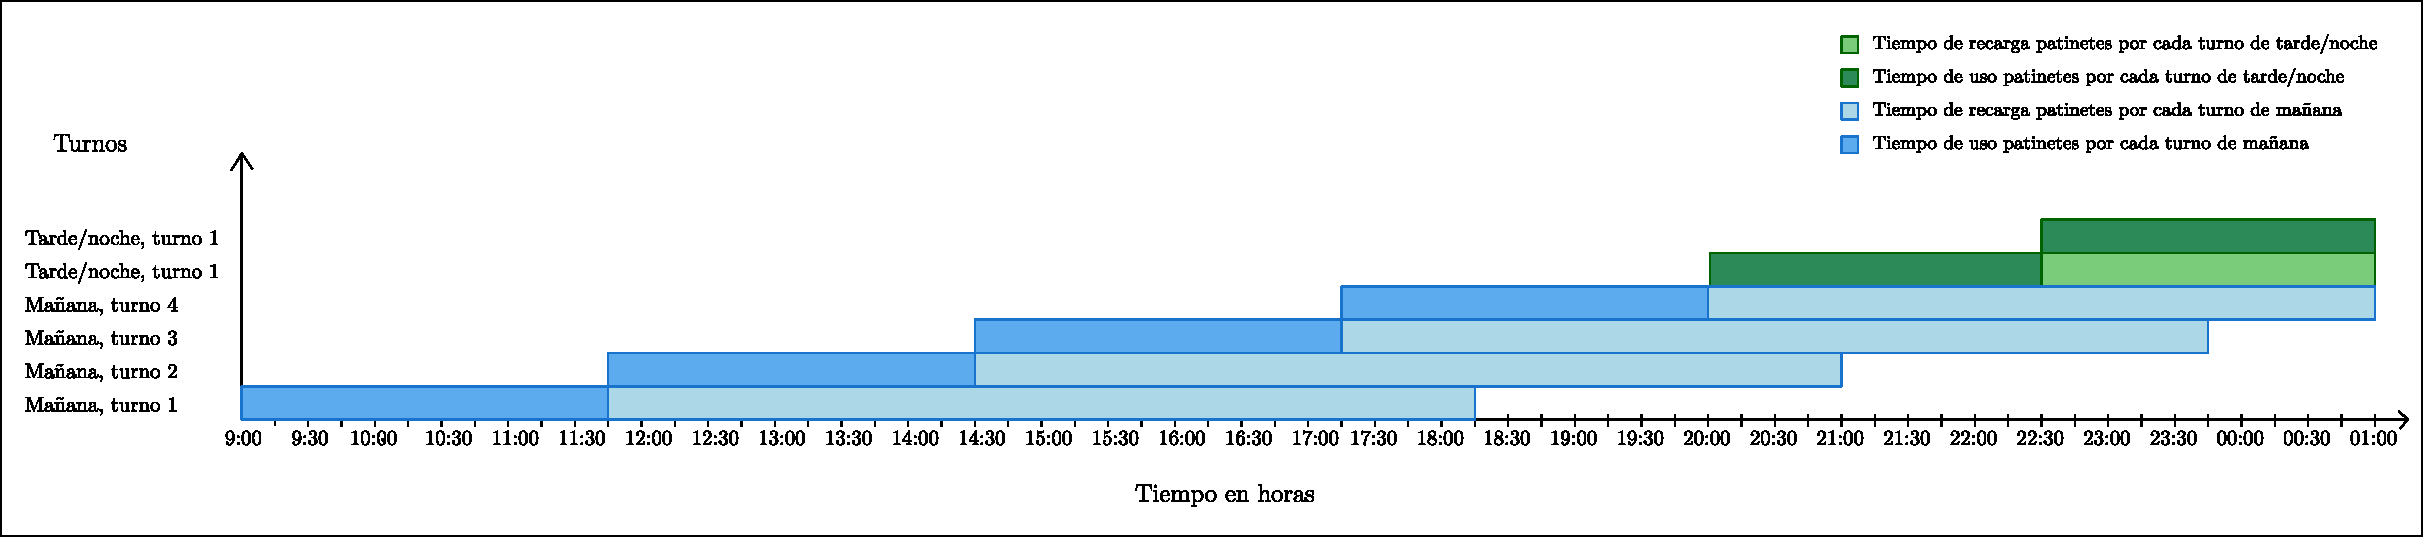
\includegraphics[width= \textwidth, height=12em]{archivos/caso1_patinetes.pdf}
    \caption{Representación turnos de patinetes en viajes de 5 \glssymbol{km}.}
    \label{fig:patinetes_caso1}
\end{figure}

La \autoref{fig:patinetes_caso1} muestra 6 turnos de vehículos, los cuatro primeros en color azul son de 2 vehículos cada uno, lo que implica que se usan 8 patinetes por la mañana. El color verde marca el comienzo del horario de tarde que estará dividido en 2 turnos, cada uno de 7 vehículos. Según el gráfico, cuatro de los vehículos de la mañana se encuentran para el segundo turno de la tarde.

Igualmente, para el supuesto de repartos dobles, recogido en la \autoref{tabla: analisis_detallado_patinete_7.5km}, son reutilizables otros cuatro patinetes, tal como queda reflejado en la
\autoref{fig:patinetes_caso2}.

\begin{figure}[ht]
    \centering
    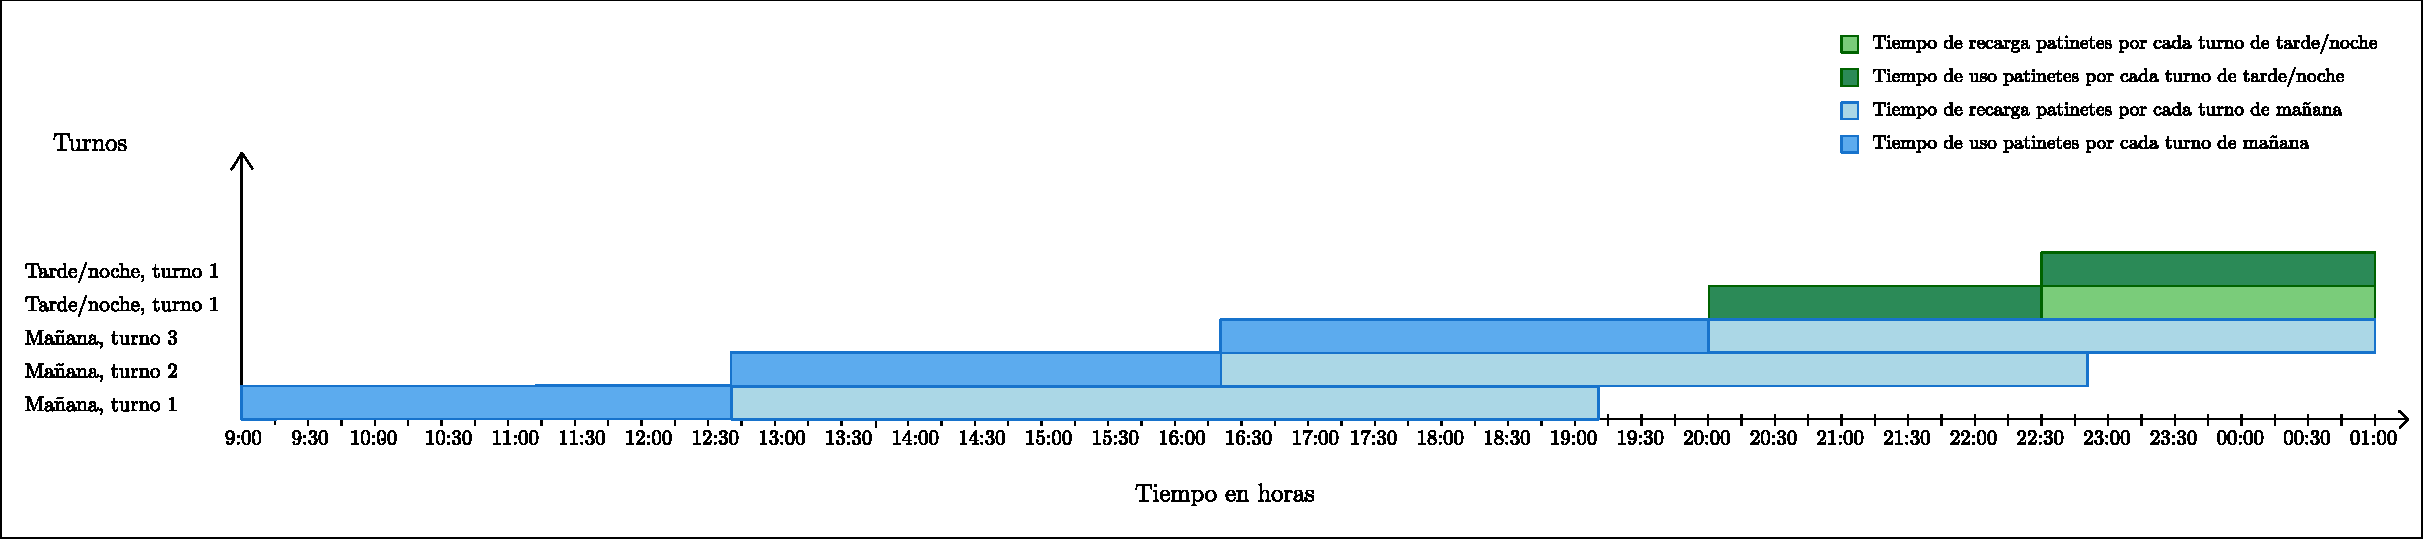
\includegraphics[width= \textwidth, height=12em]{archivos/caso2_patinetes.pdf}
    \caption{Representación turnos de patinetes en viajes de 7,5 \glssymbol{km}.}
    \label{fig:patinetes_caso2}
\end{figure}

Finalmente, se llega a la conclusión que, dada las dos hipótesis de estudios proporcionadas por la empresa, son necesarios veinte patinetes eléctricos en la primera de ellas y, para la segunda, solo dieciséis. Los resultados económicos del análisis de la Infiniton CITYJam Pro quedan reflejados en la \autoref{tab: analisis_presupuestos_patienetes}





% Formula 1
%\begin{equation}
%\label{eqn:ecuacion presupuesto patinete 5km}
 %  11550,11+2817,71*9 = 36.909,5 \text{ \glssymbol{euro}}
%\end{equation}

%\begin{equation}
%\label{eqn: ecuacion presupuesto patinete 7.5km}
%   9327,63+2251,71*9 = 29.593,2 \text{ \glssymbol{euro}}
%\end{equation}



\begin{table}[H]
\centering
\begin{tabular}{|l|c|}
\hline
N.º recargas semanales caso 1 & 136 \\ \hline
N.º recargas semanales caso 2 & 108 \\ \hline
Capacidad batería vehículo (\glssymbol{kilovatiohora}) & 0,35 \\ \hline
Coste recarga unitario (\glssymbol{euro}) & 0,04 \\ \hline
Gasto semanal en  recargas caso 1 (\glssymbol{euro}) & 5,33 \\ \hline
Gasto semanal en  recargas caso 2 (\glssymbol{euro}) & 4,23 \\ \hline
Presupuesto anual en recargas caso 1 (\glssymbol{euro}) & 277,05 \\ \hline
Presupuesto anual en recargas caso 2 (\glssymbol{euro}) & 220,01 \\ \hline
Precio unitario/vehículo (\glssymbol{euro}) & 376,62 \\ \hline
Precio unitario mantenimiento (\glssymbol{euro}) & 124,8 \\ \hline
Reserva de sustitución por vehículo (\glssymbol{euro}) & 20 \\ \hline
Presupuesto para   vehículos primer año caso 1 (\glssymbol{euro}) & 12.323,53 \\ \hline
Presupuesto para vehículos primer año   caso 2 (\glssymbol{euro}) & 9.926,05 \\ \hline
Presupuesto para vehículos anual  caso 1 (\glssymbol{euro}) & 3.873,05 \\ \hline
Presupuesto para vehículos anual caso 2 (\glssymbol{euro}) & 3.096,81 \\ \hline
Presupuesto en vehículos a 10 años, caso 1 (\glssymbol{euro}) & 47.180,97 \\ \hline
Presupuesto en vehículos a 10 años, caso 2 (\glssymbol{euro}) & 37.797,34 \\ \hline
\end{tabular}
\caption{Análisis de los presupuestos patinetes.}
\label{tab: analisis_presupuestos_patienetes}
\end{table}




